\documentclass[a4paper,11pt,titlepage]{article}
\usepackage[utf8]{inputenc} %support de l'utf8
\usepackage[T1]{fontenc} %support des accents
\usepackage[francais]{babel} %support de la langue
\usepackage{graphicx}
\usepackage{float} 

\title{AGM\\Moteur de Rendu en Lancé de Rayon}
\author{Pauline CHAMOREAU \and Nicolas RIGNAULT}


\begin{document}
\maketitle

\newpage
\section{Partie 1}

\subsection{Intersection (1.a)}

Pour calculer l'intersection du rayon avec la géométrie de la scène, on itère sur tous les triangles composants cette scène (on itère donc sur tous les objets de la scène pour récupérer tous les triangles). Pour chaque triangle, on appelle la méthode \textit{intersect\_real} qui vérifie s'il y a une intersection entre le triangle et le rayon via le calcul des coordonnées barycentriques du triangle (voir \textbf{Ray.cpp}).

Si $\beta + \gamma < 1$ et $\beta > 0$ et $\gamma > 0$ alors c'est qu'il y a bien intersection entre le rayon et le triangle. On stocke donc les coordonnées barycentriques ainsi que la distance t entre le rayon et le triangle. On continue l'itération afin de rechercher le triangle au premier plan de la scène, pour chaque pixel (on cherche donc le plus petit t). Une fois ce triangle trouvé, on lui affecte une couleur.\\

\begin{figure}[H]
 \begin{center}
 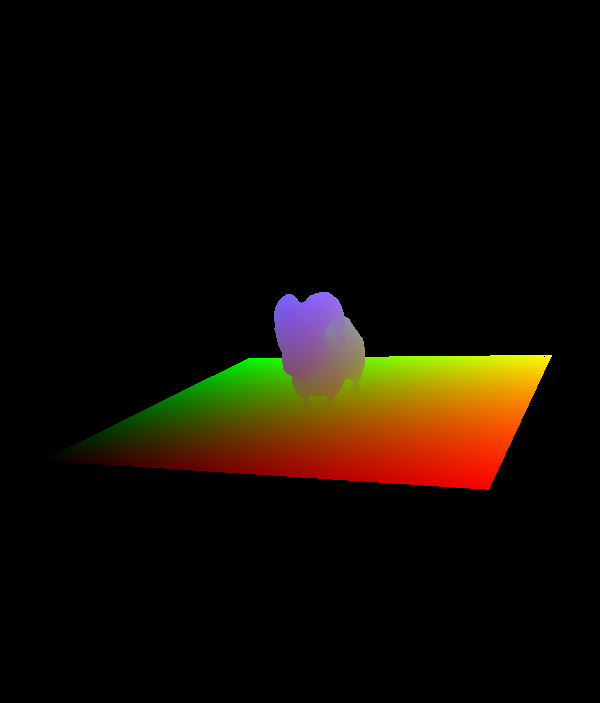
\includegraphics[bb=0 0 50 50,width=8cm]{Rendu/Intersection.png}
 \end{center}

 \caption{Rendu Bélier avec Intersection}
 \label{rendu1}
\end{figure}

Pour pouvoir utiliser ce mode, il faut cocher ``Intersection''.\\

Tout le code associé se trouve dans la méthode \textit{render} du fichier \textbf{RayTracer.cpp} (pour l'itération sur les triangles) et dans la méthode \textit{intersect\_real} du fichier \textbf{Ray.cpp} (pour le calcul de point d'intersection).

\subsection{BRDF de Phong (1.b)}

Pour calculer l'intensité lumineuse avec la BRDF de Phong, nous avons utilisé la formule $I = I_d + I_s$, $I_d$ représentant la partie diffuse de l'intensité lumineuse et $I_s$ la partie spéculaire. \\

Les calculs de $I_d$ et $I_s$ se font à l'aide des formules suivantes : \\
$I_d = k_d(\vec N \cdot \vec L)I_L$ avec 
\begin{itemize}
 \item[$k_d$ :] coefficient de reflectivité à la lumière diffuse, attribut du matériel de l'objet.
 \item[$\vec N$ :] vecteur normal à la surface, calculé à l'aide des coordonnées barycentriques du point d'intersection et des vecteurs normaux aux sommets du triangle.
 \item[$\vec L$ :] vecteur directeur de la lumière, attribut de la classe \textit{Light}
 \item[$I_L$ :] coefficient d'intensité de la lumière, aussi attribut de la classe \textit{Light}.\\
\end{itemize}
et $I_s = k_s(\vec S \cdot \vec R)^nI_L$ avec : 
\begin{itemize}
 \item[$k_s$ :] coefficient de reflectivité à la lumière spéculaire, attribut du matériel de l'objet.
 \item[$\vec S$ :] vecteur directeur de la caméra, paramètre de la fonction \textit{render}.
 \item[$\vec R$ :] vecteur directeur du rayon réfléchi, calculé avec la formule\\ $\vec R = 2(\vec L \cdot \vec N)\vec N - \vec L$.
 \item[$I_L$ :] coefficient d'intensité de la lumière, attribut de la classe \textit{Light}.\\
\end{itemize}


Pour tout pixel contenant un point d'intersection, ces calculs sont effectués pour chacune des lumières de la scène. Le $I$ calculé pour une lumière est multiplié par sa couleur ainsi que par la couleur de l'objet.\\
Pour finir, on calcule la moyenne des résultats trouvés ce qui donne la couleur effective du pixel concerné qui peut ainsi lui être appliquée.\\

\begin{figure}[H]
 \begin{center}
 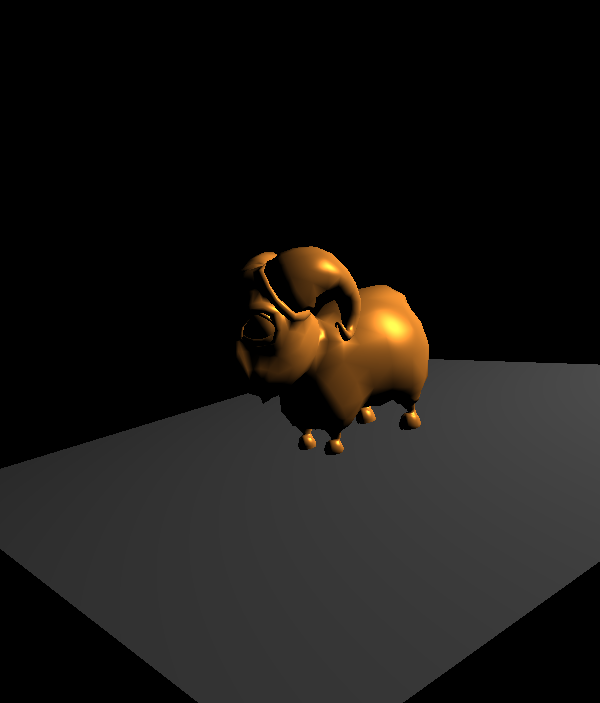
\includegraphics[bb=0 0 50 50,width=8cm]{Rendu/BRDF.png}
 \end{center}

 \caption{Rendu Bélier avec la BRDF de Phong}
 \label{rendu2}
\end{figure}

Pour pouvoir utiliser ce mode, il faut cocher ``Phong (BRDF)''.\\

Tout le code associé se trouve dans la méthode \textit{render2} du fichier \textbf{RayTracer.cpp} (pour l'itération sur les triangles et le calcul de la couleur de l'objet) et dans la méthode \textit{intersect\_real} du fichier \textbf{Ray.cpp} (pour le calcul de point d'intersection).

\newpage
\section{Partie 2}

\subsection{Ombres dures (2.a)}

On garde ce qui a été fait pour la BRDF de Phong. Cependant, on souhaite vérifier si pour chaque intersection il n'y aurait pas un triangle entre la lumière et cette même intersection. Ainsi, pour chaque intersection, on itère de nouveau sur les triangles et on vérifie s'il n'y en a pas un entre la lumière et l'intersection (pour cela, on lance un rayon ayant pour origine la lumière, en direction de l'intersection trouvée précédemment).

Si on trouve bel et bien une intersection, alors le triangle est caché et on doit générer une ombre (on change la couleur du pixel). Sinon, on garde la couleur associée au triangle.\\

\begin{figure}[H]
 \begin{center}
 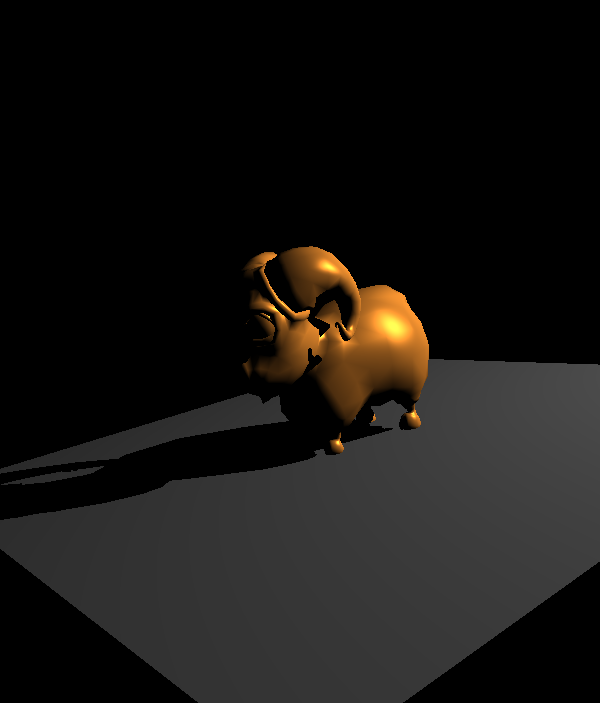
\includegraphics[bb=0 0 50 50,width=8cm]{Rendu/OmbresD.png}
 \end{center}

 \caption{Rendu Bélier avec les Ombres dures}
 \label{rendu3}
\end{figure}

Pour pouvoir utiliser ce mode, il faut cocher ``Ombres dures''.\\

Tout le code associé se trouve dans la méthode \textit{render3} du fichier \textbf{RayTracer.cpp} (pour l'itération sur les triangles et le calcul de la couleur de l'objet ainsi que des ombres) et dans la méthode \textit{intersect\_real} du fichier \textbf{Ray.cpp} (pour le calcul de point d'intersection).


\subsection{Ombres douces (2.b)}

On garde les bases de l'algorithme pour les ombres douces. On ajoute seulement un tableau comprenant les différents rayons que l'on souhaite lancer. On choisit d'en rajouter 12 tout autour de la source lumineuse (le 13\up{e} étant lancé depuis l'origine de la lumière). 

Une fois tous les rayons lancés, on itère à nouveau sur tous les triangles pour chercher une intersection différente de celle que l'on a trouvée. Si on trouve une telle intersection, on incrémente un flottant qui sera appliqué sur la lumière pour l'adoucir.\\

Cette méthode comporte quelques erreurs car on n'obtient pas tout à fait le rendu espéré.

\begin{figure}[H]
 \begin{center}
 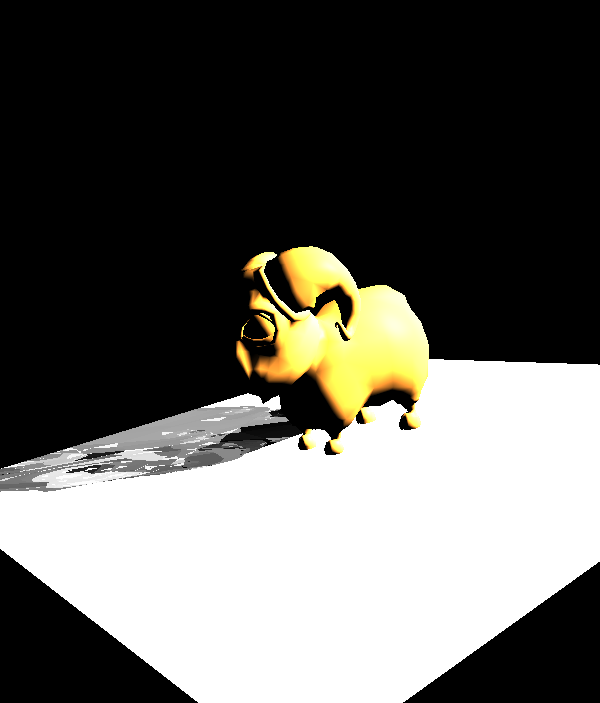
\includegraphics[bb=0 0 50 50,width=8cm]{Rendu/OmbresD2.png}
 \end{center}

 \caption{Rendu Bélier avec les Ombres douces (test)}
 \label{rendu4}
\end{figure}

Pour pouvoir utiliser ce mode, il faut cocher ``Ombres douces''.\\

Tout le code associé se trouve dans la méthode \textit{render4} du fichier \textbf{RayTracer.cpp} (pour l'itération sur les triangles et le calcul de la couleur de l'objet ainsi que des ombres) et dans la méthode \textit{intersect\_real} du fichier \textbf{Ray.cpp} (pour le calcul de point d'intersection).


\section{Manuel}

L'interface du RayTracer a été modifiée afin de pouvoir être manipulée facilement. Au lancement du programme, il faut donc faire plusieurs choix:
\begin{itemize}
 \item Activation ou non de la Haute Définition (très lent)
 \item Utilisation du plan où reposent le(s) objet(s)
 \item Choix de la scène (Bélier ou Sphère)\\
\end{itemize}

L'activation des différentes méthodes de rendu se fait ensuite via la sélection des boutons se trouvant sous le bouton ``Render'':
\begin{itemize}
 \item ``Intersection'': rendu correspondant à la question 1.a
 \item ``Phong (BRDF)'': rendu correspondant à la question 1.b
 \item ``Ombres dures'': rendu correspondant à la question 2.a
 \item ``Ombres douces'': rendu correspondant à la question 2.b
\end{itemize}

\section{Meilleur rendu}

Le meilleur rendu que nous somme parvenus à obtenir est celui pour les Ombres dures.
Le KD-Tree n'a pas été implémenté et le rendu avec les Ombres douces ne fonctionne pas correctement.

\begin{figure}[H]
 \begin{center}
 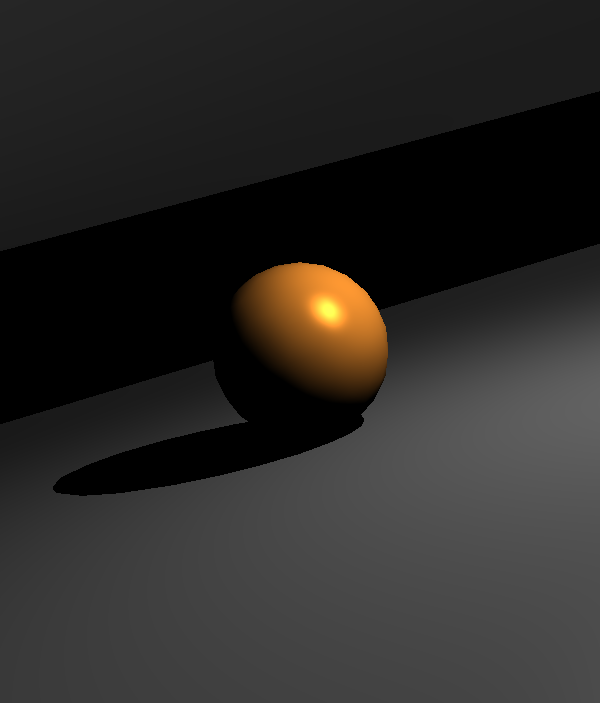
\includegraphics[bb=0 0 50 50,width=8cm]{Rendu/OmbresDS.png}
 \end{center}

 \caption{Rendu Sphère avec les Ombres dures}
 \label{rendu5}
\end{figure}


\end{document}
